\documentclass{article}


% if you need to pass options to natbib, use, e.g.:
%     \PassOptionsToPackage{numbers, compress}{natbib}
% before loading neurips_2023
% ready for submission
\usepackage[preprint]{neurips_2023}


% to compile a preprint version, e.g., for submission to arXiv, add add the
% [preprint] option:
%     \usepackage[preprint]{neurips_2023}


% to compile a camera-ready version, add the [final] option, e.g.:
%     \usepackage[final]{neurips_2023}


% to avoid loading the natbib package, add option nonatbib:
%    \usepackage[nonatbib]{neurips_2023}
\usepackage{commands}




\title{Expected Gradient Estimator With Many Environments}


% The \author macro works with any number of authors. There are two commands
% used to separate the names and addresses of multiple authors: \And and \AND.
%
% Using \And between authors leaves it to LaTeX to determine where to break the
% lines. Using \AND forces a line break at that point. So, if LaTeX puts 3 of 4
% authors names on the first line, and the last on the second line, try using
% \AND instead of \And before the third author name.


\author{%
  Navid Ardeshir \\
  Department of Statistics\\
  Columbia University \\
  \texttt{navid.ardeshir@columbia.edu} \\
}


\begin{document}


\maketitle


\begin{abstract}
    In this paper we deal with the problem of finding an invariant subspace where the regression function only varies in that subspace across different environments.
    This problem can also be thought of as a representation learning with nonlinear link function.
    Inspired by ideas in the sufficient dimension reduction literature \citep{li2018sufficient} and recent developments in multi-task learning \citep{boursier2022trace} we propose a novel method which exploits data from all environments and provide numerical evidence for its tractability. 
\end{abstract}

\section{Introduction}
Consider the setting where we have observed datasets from multiple environments $\environments$. 
Each dataset $\dataset[e] := \left\{ (X_{i}^{e}, Y_{i}^{e}) : i \leq n_e \right\} \subset \mathcal{X} \times \mathcal{Y}$ contains $n_e$ samples from the population distribution $\probability[e] \in \mathcal{P}(\mathcal{X} \times \mathcal{Y})$ where $e \in \environments$. 
In particular, we impose certain parametric assumptions over these distributions, that is, the response variable $Y^{e}$ are only related to the covariates $X^e$ through a linear subspace that is invariant among different environments.
In other words, there exists a matrix $B \in \mathbb{R}^{d \times k}$ where $ Y^{e} \indep X^{e} \given {B}^{\T} X^{e} $, and thus, the rgeression function satisfies $ \expectation{ Y^{e} \conditional X^{e} } = \expectation{ Y^{e} \conditional B^{\T} X^{e} } $.
Although, the matrix $B \in \mathbb{R}^{d \times k}$ is not necessarily identifiable, but classical sufficient dimension reduction methods allows us to recover the column space of $B$ denoted by $\mathscr{L} = \spn\{ B_{i} \in \mathbb{R}^{d} : 1 \leq i \leq k \} = \col(B)$ which we also call central subspace. 
Our goal in this article is to recover this central subspace by taking advantage of datasets from different environments, enabling out of distribution generalization in unseen environments with similar representations with very few samples.

Estimating the regression function under such structures are indeed more amenable and adaptive, especially when we are dealing with high dimensional datasets such that $k \ll d$, as the number of necessary samples only grows with the subpace dimension $k$ as opposed to the ambient dimension $d$ \citep{xia2002adaptive} 
and even parametric rates are achievable under further distributional assumptions \citep{yuan2023efficient}.
These approaches enjoy their adaptivity property owing to: 
\begin{enumerate}[label=(\roman*)]
    \item learning the invariant subspace, enabling to project data onto a low dimensional subspace.
    \item estimate the regression function in the projected subspace.
\end{enumerate}
Note that generalization to unseen environments with only few samples is a simple consequence of reusing the invariant subspace in observed environments which can be learned by samples from the observed environments.
In the following we focus on the first part and elaborate on a famously used method for learning the central subspace known as Expected Gradient Outerproduct \citep{li2018sufficient, hristache2001direct}. 
Assuming the regression function $f_e: \mathbb{R}^k \to \mathbb{R}: z \mapsto \expectation{Y^{e} \conditional B^{\T}X^{e} = z}$ is differentiable and denoting $Z^{e} = B^{\T} X^{e}$ to be the latent variable then the main observation is that the gradient of the regression function is in the desired central subspace
, i.e. $ \nabla_{x} f_e (B^{\T}X^{e}) = B \nabla_z f_e(Z^{e}) \in \mathscr{L}$. Taking the average over the poppulation distribution yields expected gradient outer product (EGOP),
$$ M^{e, e} := \expectation{ \nabla_x f_e( B^{\T}X^{e}) \nabla_x^{\T} f_e( B^{\T} X^{e}  ) } = B \expectation{ \nabla_z f_e( Z^{e}) \nabla_z^{\T} f_e( Z^{e}  ) } B^{\T} \in \mathbb{R}^{d \times d} $$
Indeed the central subspace $\mathscr{L}$ is inclusive of columns space of $M^{e}$ and equality only holds if the latent gradient average outerproduct $\expectation{ \nabla_z f_e( Z^{e}) \nabla_z^{\T} f_e( Z^{e}  ) } \in \mathbb{R}^{k \times k}$ is invertible. 
Under this condition which can be shown to be equivalent to $\mathscr{L}= \col(B)$ being the smallest subspace for which the regression function only varies in directions of columns of $B$, then the central subspace $\mathscr{L}$ can be identified.
Interestingly one can take advantage of other datasets and take average gradient outer product with respect to other measures to recover the central subspace more accurately so long as the resulting latent gradient outer product is inveritble. 
This naturally leads to defining,
$$ M^{e, e'} := \expectation{ \nabla_x f_e( B^{\T}X^{e'}) \nabla_x^{\T} f_e( B^{\T} X^{e'}  ) } = B \expectation{ \nabla_z f_e( Z^{e'} ) \nabla_z^{\T} f_e( Z^{e'}  ) } B^{\T} \in \mathbb{R}^{d \times d}  $$
where the gradient outer product is obtained from model in environment $e \in \environments$ but evaluated at enviromnet $e' \in \environments$.
Indeed, each individual EGOP can be used for recovering the central subspace, but the remaining challenge is how to combine them.

\paragraph*{Our Method:} We propose an estimator for central subspace using singular value decomposition of the following matrix,
\begin{equation*}
    M^{\environments \times \environments} = 
    \begin{bmatrix}
        M^{e_1,e_1} & \dots & M^{e_1,e_T} \\
        M^{e_2, e_1} & \dots & M^{e_2, e_T} \\
         & \vdots & \\
        M^{e_T, e_1} & \dots & M^{e_T,e_T} \\
    \end{bmatrix}
    \in \mathbb{R}^{ dT \times dT }
\end{equation*}
where $T = \abs{\environments}$ is the number of observed environments. 
This matrix, under the invariant subspace assumption has low rank (less than $k$) and captures the interactions across different environments.
%One hopes to recover the central subspace using $M^{\environments \times \environments}$ more robustly and efficiently given that it captures the interactions across different environments 
%However, estimating the central subspace based on this matrix $M^{\environments \times \environments}$ is less direct that of its submatrices $M^{e}$ as we can simly use $\col\left( M^{e} \right)$.
%To that end, we propose an estimator for central subspace using singular value decomposition of the matrix $M^{\environments \times \environments}$. 
More formally, let $r = \operatorname{rank}\left( M^{\environments \times \environments} \right)$ be the rank of this matrix then we have the following decomposition,
\begin{equation*}
    M^{\environments \times \environments} = U^{\environments} \Lambda {V^{\environments}}^{\T} =
    \begin{bmatrix}
        U_1^{e_1} & \dots & U_r^{e_1} \\
        U_1^{e_2} & \dots & U_r^{e_2} \\
        & \vdots & \\
        U_1^{e_T} & \dots & U_r^{e_T} \\
    \end{bmatrix}
    \begin{bmatrix}
        \lambda_1 & & & \\
        & \lambda_2 & & \\
        & & \ddots & \\
        & & & \lambda_r \\
    \end{bmatrix}
    \begin{bmatrix}
        V_1^{e_1} & \dots & V_r^{e_1} \\
        V_1^{e_2} & \dots & U_r^{e_2} \\
        & \vdots & \\
        V_1^{e_T} & \dots & V_r^{e_T} \\
    \end{bmatrix}^{\T}
\end{equation*}
where $U^{\environments}_i = [{U_i^{e_1}}^{\T}, {U_i^{e_2}}^{\T}, \dots, {U_i^{e_T}}^{\T}]^{\T} \in \mathbb{S}^{dT} $ are orthonormal vectors (of length one) in column space of $M^{\environments \times \environments}$ with $U_i^{e_j} \in \mathbb{R}^d$, 
and similarly $V^{\environments}_i = [{V_i^{e_1}}^{\T}, {V_i^{e_2}}^{\T}, \dots, {V_i^{e_T}}^{\T}]^{\T} \in \mathbb{S}^{dT} $ are orthonormal vectors (of length one) in row space of $M^{\environments \times \environments}$ with $U_i^{e_j} \in \mathbb{R}^d$. 
Finally, we estimate the central subspace using the column space of the following matrix,
\begin{equation*}
    \col \left( 
    \begin{bmatrix}
        \frac{1}{T} \sum_{e \in \environments}\frac{U_1^{e}}{ \norm{U_1^{e}} }, & \dots & , \frac{1}{T} \sum_{e \in \environments} \frac{U_k^{e}}{ \norm{U_k^{e}} } 
    \end{bmatrix}
    \right)
\end{equation*}
The normalization is in fact crucial in our setting and we suspect it acts as some form of "debiasing" (see Section 3 for further detail).
 





\section{Preliminaries}
\subsection{Sufficient Dimension Reduction}
Our focus in this work is to estimate the shared central subspace among various environments. 
In the following we proceed to formally define this subspace and specify some of its properties. 

\begin{definition}[Central subspace]
    For a pair $(X,Y)$ distributed according to $\probability \in \mathcal{P}(\mathcal{X} \times \mathcal{Y})$ we define the central subspace as the smallest subspace for which the regression function $\expectation{Y \conditional X}$ only varies in that subspace, i.e.
    $$ \mathscr{L} := \bigcap \left\{ \col\left( B \right) \subseteq \mathbb{R}^{d} : \expectation{Y \conditional X} = \expectation{Y \conditional B^{\T} X} \,\, \probability \text{-almost-everywhere} \right\} $$
    where $\col(\cdot)$ represent the column space of its argumnet.
\end{definition}

The existence of such a subspace can be guaranteed under mild assumptions over the support of $X$ (see \citep{li2018sufficient} for further details). 
As discussed earlier the minimality assumption on the central subpace is crucial and implies its identifiability. 

\begin{proposition}[identifiability of central subapce adopted from \citep{li2018sufficient}]
    \label{prop:identifiability}
    Suppose the regression function for $(X,Y) \sim \probability$ denoted by $f: \mathcal{X} \to \mathcal{Y}:x \mapsto \expectation{Y \conditional X = x}$ is differentiable. Then, the central subspace $\mathscr{L}$ associated with $\probability$ defined in \ref{def:grasssmanian-distance} satisfies the following:
    \begin{enumerate}[label=(\roman*)]
        \item The gradient of the regression function is in the central subspace at almost every point and,
        $$ \operatorname{ Support }( \nabla_x f(X) ) = \mathscr{L} $$
        \item The central subspace can be recovered from the column space of the average gradient outer product (EGOP) matrix,
        $$ \col \left(\expectation{ \nabla_x f(X) \nabla_x^{\T} f(X) } \right) = \mathscr{L} $$
    \end{enumerate} 
\end{proposition}
We omit the proofs for Proposition \ref{prop:identifiability} (see \citep{li2018sufficient} Theorem 11.1). 
We may now state our central assumption.
\begin{assumption}[Invariant central subspace]
    \label{assum:invariance}
    A collection of probability distributions $(\probability[e])_{e \in \environments}$ have invariant central subspaces if their corresponding central subspaces are all equal, i.e.
    $$ \mathscr{L}^e = \mathscr{L} \quad \quad \forall e \in \environments $$
\end{assumption}
Although this assumption may seem to be strong, our numerical experiments demonstrates robustness to small deviations of this assumption where a few of the environments do not share the same central subspaces.

In the sequel we take $P_{\mathscr{L}} \in \mathbb{R}^{d \times d}$ to be the projection matrix onto the central subspace and let $k = \operatorname{tr}(P_{\mathscr{L}}) = \operatorname{dim}(\mathscr{L})$ to be the dimension of the central subspace and assume its value is known to the statistian.\footnote{We later discuss further how can one estimate the value of $k = \operatorname{\mathscr{L}}$ using data.}
In order to evaluate the performance of an estimator for the central subspace we use the following distance.
\begin{definition}[Grassmanian distance]
    \label{def:grasssmanian-distance}
    For a pair of subspces $\hat{\mathscr{L}}, \mathscr{L} \subseteq \mathbb{R}^d$ of dimension $k$ we define the grassmanian distance using their projection matrices $P_{\mathscr{L}}, P_{\hat{\mathscr{L}}} \in \mathbb{R}^{d \times d}$ as,
    $$ d(\hat{\mathscr{L}}, \mathscr{L}) := \norm[\operatorname{Fr}]{ P_{\hat{\mathscr{L}}} - P_{\mathscr{L}} } = \sqrt{ \operatorname{tr}\left( \left( P_{\hat{\mathscr{L}}} - P_{\mathscr{L}} \right)^2 \right) } $$
\end{definition}
\begin{remark}
    We remark that this distance is closely related to $\sin \theta(\cdot, \cdot)$ distance commonly used in the literature where $\theta(\cdot, \cdot)$ represents the principal angles between the two subspaces. More formally, for $i \leq k$ the $i$'th principal angle corresponds to
    $$ \sin^2 \theta_i(\hat{\mathscr{L}} , \mathscr{L}) = \lambda_i\left( \left( P_{\hat{\mathscr{L}}} - P_{\mathscr{L}} \right)^2 \right) $$
    where $\lambda_i(\cdot)$ denotes the $i$'th eigenvalue of its argument. Thus, the distance defined in \ref{def:grasssmanian-distance} corresponds to $\sqrt{\sum_{i = 1}^{k} \sin^2 \theta_i}$ and accounts for all principal angles.
\end{remark}

\subsection{Non-parametric Estimation of Gradient Outer Product}
In this section we demonstrate how we can estimate the central subspace using non-parametric kernel regression methods.

Suppose $\hilbert_h$ is a reproducing kernel hilbert space induced from kernel $K_h:\mathcal{X} \times \mathcal{X} \to \mathbb{R}$ indexed by a tunable bandwidth parameter $h > 0$. 
In particular we use the radial basis kernel $K_h:(x,x') \mapsto h^{-d/2} \exp( -\frac{ \norm[2]{x - x'} }{2 h^2} ) $. 
Given a dataset $\dataset = \left\{ (X_i, Y_i) : i \leq n \right\}$ where $(X_i, Y_i) \sim \probability$ we define the regularized kernel estimator as,
$$ \hat{f}_{\eta, h} = \arg\min_{f \in \hilbert_h} \sum_{i=1}^{n} (Y_i - f(X_i))^2 + \eta \norm[ \hilbert_h ]{f}^2 $$
which can be explicitly written using Mercer's theorem as,
$$ \hat{f}_{\eta, h}(\cdot) = \sum_{i=1}^{n} \hat{\alpha}_i K(\cdot, X_i) ,\quad\quad \hat{\alpha} = \left( K_h(X, X) + \eta \mathbb{I}_{n \times n} \right)^{-1} Y \in \mathbb{R}^{n} $$ 
%where $\hat{\alpha}^e \in \mathbb{R}^{n_e}$ satisfies the normal equations,\footnote{Note that we are dropping the dependence of $\hat{\alpha}^e$ on the regularization parameter $\eta_e$ for notational convenience.}
%$$ \hat{\alpha}^{e} = \left( K(X^e, X^e) + \eta_e \mathbb{I}_{n_e \times n_e} \right)^{-1} Y^e $$
where $K_h(X,X) = (K_h(X_i, X_j))_{i,j} \in \mathbb{R}^{n \times n}$ is the kernel covariance matrix. Our EGOP estimate can be obtained via,
$$ \hat{M}_{\eta, h} := \frac{1}{n} \sum_{i=1}^{n} \nabla_x \hat{f}_{\eta, h}(X_i) \nabla^{\T}_x \hat{f}_{\eta, h}(X_i) $$
Although, non-asymptotic rates for the regularized kernel estimator exists (e.g. \citep{bach2017breaking} for a specific ReLU kernel), we are unaware of sample complexity guarantees for the EGOP estimate defined above, that is how many samples are needed so that $\hat{M}_{\eta,h}$ to be sufficiently close to the true expected gradient outer product.
Existing results mostly deal with Nadaraya-Watson type estimates (e.g. \citep{yuan2023efficient, trivedi2014consistent}) or local linear regression approaches (e.g. \citep{wu2010learning}) as opposed to inverse methods where the regression coefficients are obtained from the inverse of a matrix. 
However we use inverse methods due to their practical superiority.
It is worth reiterating that we are merely concerned about consistency of the column space of the estimated EGOP matrix, and consistently estimating the regression function is not of essence in our setting.
%Moreover, our approach described in the introduction can be thought of as a meta approach which combines a collection of estimates of EGOPs with shared structure and can be applied to other estimators for EGOP.

We use kernel regression described above to obtain an estimate regression function for each environment and then form its corresponding EGOP matrices.
Using sample splitting schemes we tune the hyperparameters, namely, regularization parameter $\eta_e$, and kernel bandwidth $h_e$, for each individual environment $e \in \environments$ and denote the regression function estimates as $\hat{f}_e$ (see Appendix for further details). 

\begin{definition}[EGOP estimation per environment]
    \label{def:egop-per-env}
    Given datasets $\dataset[e] = \left\{ (X_i^e, Y_i^e): i \leq n_e \right\}$ where $(X_i^e, Y_i^e) \sim \probability[e]$ and it's esimate regression function $\hat{f}_e$ described above we obtain the expected gradient outer product estimates using,
    $$ \hat{M}^{e,e'} := \frac{1}{n_{e'}} \sum_{i=1}^{n_{e'}} \nabla_x \hat{f}_{e}(X_i^{e'}) \nabla^{\T}_x \hat{f}_{e}(X_i^{e'}) \in \mathbb{R}^{d \times d}, \quad\quad \forall e,e' \in \environments $$
    Moreover, we define $\hat{\mathscr{L}}^{e,e'} = \col\left( \hat{M}^{e,e'} \right)$ to be an estimate for central subspace corresponding to $\probability[e]$.
\end{definition}



% \section{Related Works}
% \paragraph*{Multitask Learning:}
Our setting also can be viewed as multi-task learning which has been more extensively studied in the linear settting. In particular, the works of \citep{boursier2022trace} impose a low rank assumption on the coefficient matrix (simillar to ours)

\paragraph*{Transfer Learning:}

\paragraph*{Causal Representation Learning:}


\section{Estimating the Central Subspace with Many Environments}
In this section we first provide a naive approach for estimating the central subspace under the invariance assumption \ref{assum:invariance}.
We then elaborate on our proposed method and comment on its differences with the naive approach.

Consider a prior weight vector $w \in \mathbb{R}_{+}^{\abs{\environments}}$ over the environments satisfying $\sum_{e \in \environments} w_e = 1$.
In order to use the information from all environments and all models we aggregate the EGOP matrices using the prior $w$ and define,
$$ M^{w} := \sum_{e,e' \in \environments} \sqrt{w_e} \sqrt{w_{e'}} M^{e,e'} = U^{w} \Lambda^w {V^{w}}^{\T} \in \mathbb{R}^{d \times d}  $$
where the second equality is its singular value decomposition. In the following we establish that this aggreagation provides a feasible estimator for the central subspace.
\begin{proposition}
    \label{prop:weighted-aggregation}
    Under the invariant assumption \ref{assum:invariance} the column space of the weighted aggregated EGOP $M^{w}$ recovers the central subspace, i.e.
    $$ \col\left( M^{w} \right) = \col\left( U^{w} \right) = \mathscr{L} $$
\end{proposition}
The proof is a simple extension of Proposition \ref{prop:identifiability} and we defer it to appendix. 
Although, the choice of prior doesn't explicitly play a role in Proposition \ref{prop:weighted-aggregation}, however, it can be crucial in finite sample estimates.
This is because one expects the convergence rates for EGOP estimates to their population counterparts, i.e. $\hat{M}^{w} \to M^{w}$ when $n_e \to \infty$, to depend on the ill-conditioning of $M^{w}$,
that is how far the $k$'th largest ingular value is from the largest. The optimal choice of prior can remedy this, yet it is unknown to the statistician apriori.
We define our finite-sample naive estimator in the following using a fixed weighting choice. 
\begin{definition}[Naive estimator]
    Suppose $\hat{M}^{e,e'} \subset \mathbb{R}^{d \times d}$ to be EGOP estimates defined in \ref{def:egop-per-env} for a pair of environments $e,e' \in \environments$. 
    Then the naive estimator for central subspace can be obtained from column space of $\hat{M}^w$ with uniform prior $w_e = \frac{1}{T}$,
    $$ \hat{\mathscr{L}}^{\operatorname{naive}} = \col\left( \hat{M}^w \right)$$
\end{definition}

In order to put this estimator into perspective we resort to an optimisation representation of singular value decomposition.
Recall that the $i$'th singular vector of a matrix can be iteratively constructed based on previous singular vectors using the following optimization problem,
\begin{equation*}
    (U_i^w, V_i^w) = \operatorname*{arg\,max}_{ \substack{u,v \in \mathbb{S}^{d} \\ \forall j < i,\, u^{\T} U_j^{w} = 0 \\ \forall j < i,\, v^{\T} V_j^{w} = 0} } u^{\T} M^w v = \sum_{e,e' \in \environments} \sqrt{w_e} u^{\T} M^{e,e'} v \sqrt{w_{e'}}
\end{equation*}
This is in contrast to our approach which solves a more flexible optimization problem with less constraints but tunes the weights,
\begin{equation*}
    (U_i^{\environments}, V_i^{\environments}) = \operatorname*{arg\,max}_{ \substack{u^{e},v^{e} \in \mathbb{S}^{d} \\ \forall j < i,\, \sum_{e \in \environments}  {u^e}^{\T} U_j^{e} = 0 \\ \forall j < i,\, \sum_{e' \in \environments} {v^{e'}}^{\T} V_j^{e'} = 0} } \sum_{e,e' \in \environments} {u^e}^{\T} M^{e,e'} {v^{e'}} 
\end{equation*}
In other words the naive estimator can be thought of as a form of parameter sharing where $u^{e} = \sqrt{w^{e}} u$ and $v^{e} = \sqrt{w^e} v$ for all envrionments $e \in \environments$. This constraint might be benficial in the presence of a shared structure however the advantage of our method is that it also optimally tunes the weights to aggregate different environments.

\begin{figure}[t!]
    \label{fig:results}
    \centering
    \begin{minipage}{0.5\textwidth}
        \centering
        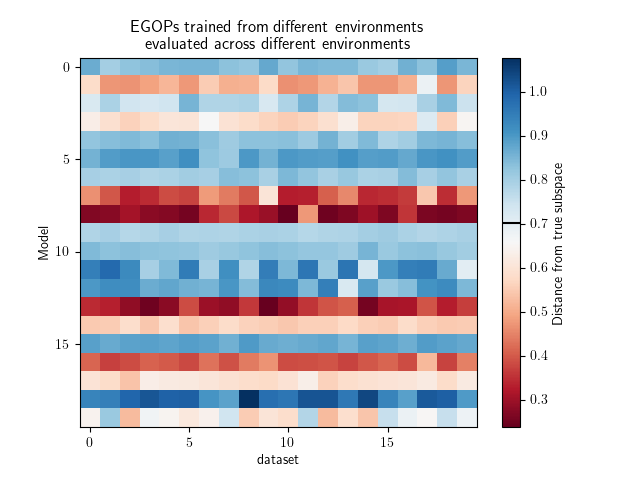
\includegraphics[width=\textwidth]{individual_performance.png}
    \end{minipage}
    \begin{minipage}{0.45\textwidth}
        \centering
        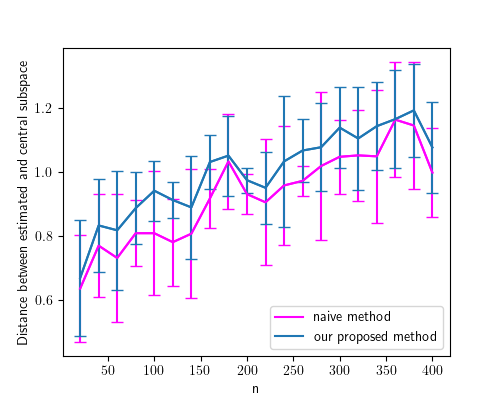
\includegraphics[width=\textwidth]{final_res.png}
    \end{minipage}
    \caption{(left) The performance of subspace estimates $\hat{\mathscr{L}}^{e,e'}$ based on individual EGOPs $\hat{M}^{e,e'}$. Rows represent the model index and columns represent the dataset which is evaluated on. 
    (right) The performance of our method on average dominates the naive method performance.}
\end{figure}



\section{Conclusion}
In this paper we deal with the problem of reducing the dimenionality of the data and finding an invariant subspace among different environments.
This problem can be indeed challenging as the regression function for each environment is nonlinear and may differ arbitrarily. 
Our setting also have close ties to multi-task and meta learning and inspired by these literatures we propose a novel method for finding such subspaces. 
Finally we empirically validate our method and compare it with classical methods from sufficient dimension reduction literature.



\bibliographystyle{plainnat}
\bibliography{bibliography}

\section{Appendix}
\subsection{Numerical Experiments}

In this section we elaborate on our synthetic setting and provide evidence for admissability of our method in comparison to the naive method.
Our codes can be found at \href{https://github.com/scO0rpion/Fields-Experiment-Project}{https://github.com/scO0rpion/Fields-Experiment-Project}.

\begin{figure}[h!]
    \centering
    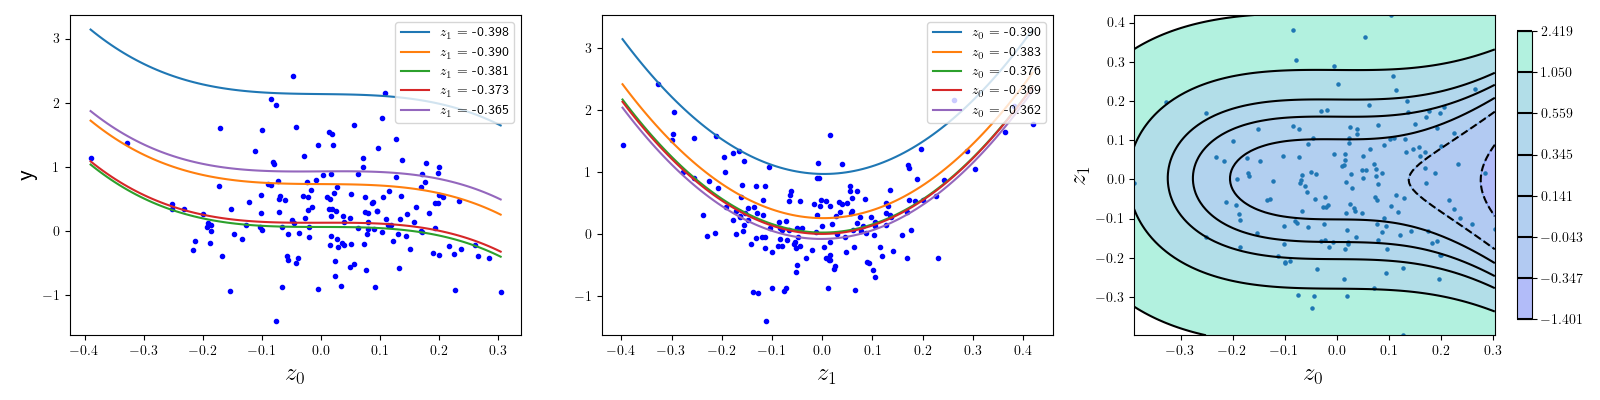
\includegraphics[width=\textwidth]{regression_fcn.png}
    \caption{Demonstrates the regression function $f_e(z_0, z_1)$ for a particular environment. The dots correspond to latent data points $(Z^{e}_i, Y^{e}_i)$ projected onto the underlying central subspace, i.e. $Z^{e}_i = B^{\T} X^{e}_i$. (left) The lines correspond to the graph of $z_0 \mapsto f(z_0,z_1)$ for different values of $z_1$. 
    (middle) The lines correspond to the graph of $z_1 \mapsto f(z_0,z_1)$ for different values of $z_0$.
    (right) The contour plot of the regression function $f_e$.}
\end{figure}

\begin{figure}[h!]
    \label{fig:singular}
    \centering
    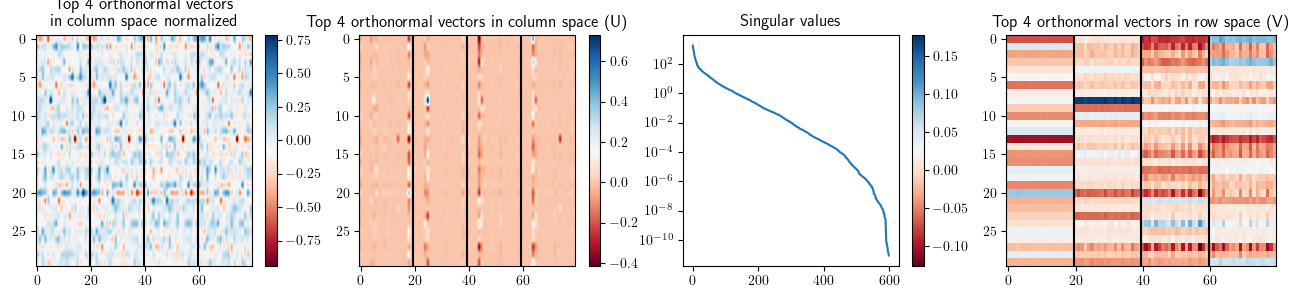
\includegraphics[width=\textwidth]{svd.png}
    \caption{An illustration of singular value decomposition of $M^{\environments \times \environments} = U^{\environments} \Lambda {V^{\environments}}^{\T}$. Top 4 singular vectors separated by black lines. Each singular vector $U^{\environments}_i \in \mathbb{R}^{dT}$ is reshaped into matrix in $\mathbb{R}^{d \times T}$ where $e$'th column represents $U_i^e$.
    (left) Each column is normalized to have length one. (left middle) Vectors in column space of $M^{\environments \times \environments}$. (right midle) Singular values demonstrate a sharp decay verifying $M^{\environments \times \environments}$ is of low rank. (right) Vectors in row space of $M^{\environments \times \environments}$. }
\end{figure}

Recall that our goal in this paper is to accurately recover the invariant central subspace using datasets from different environments. 
We generate our central subspace unfiromly at random among $k=2$ dimenional subspaces in $\mathbb{R}^{d}$ with ambient dimension $d = 30$, i.e. $\mathscr{L} = \col(B)$ where entries of $B \in \mathbb{R}^{d \times k}$ are generated from standard gaussian. 
Note that we assume the knowledge of the instrinsic dimension $k$ throughout. This value can also be estimated based on how fast the singular values of $M^{\environments \times \environments}$ drops (see Figure \ref{fig:singular}). 
We generate $T = 20$ environments for which their corresponding distribution $\probability[e]$ is obtained in the following way:
\begin{enumerate}
    \item \textbf{Random Design:} The covariates follows anisotropic gaussian $X^{e} \sim \mathcal{N}(0, \fracl{\Sigma^e}{\sqrt{d}})$ where $\Sigma^e$ is diagonal with diagonal elements following standard chi distribution.
    Similar results can be obtained when the covariates are isotropic. 
    \item \textbf{Polynomial Regression Function:} We consider a polynomial regression function with random coefficient generated from standard cauchy,
    $$ f_e(z) = a_0^e z_0^4 + a_1^e z_1^2 + a_2^e z_0 z_1$$
    \item \textbf{Homogenous Noise:} Our response variable is obtained as $Y^e = f_e(B^{\T} X^{e}) + \epsilon^e$ where the noise is gaussian with variance $\sigma = 0.5$.
\end{enumerate}
We generate datasets $\dataset[e]$ with $n$ samples from each environment and fit a regression function estimator $\hat{f}_e$ using kernel regression with a RBF kernel. Additionally we perform a 80-20 percent sample splitting to tune the hyperparameters.
Finally, we evaluate the performance of our algorithm averaged over 20 experiments for each choice of sample size $n$ and demonstrate the results in Figure~\ref{fig:results}.






\end{document}